\documentclass{article}
\usepackage[margin=1in]{geometry}
\usepackage{booktabs}
\usepackage{enumitem}
\usepackage{tikz}
\usepackage{graphicx}
\usepackage{lipsum}
\usepackage{caption}
\usepackage{subcaption}

\title{Demo LaTeX File}
\author{TeXtra Assistant}
\date{\today}

\begin{document}

\maketitle

\section{Introduction}
This is a demonstration LaTeX file showcasing various environments such as tables, lists, and figures. The following sections contain examples that span approximately ten pages when compiled with standard formatting.

\lipsum[1-3]

\section{Tables}
Here we present a simple table using the \texttt{booktabs} package for professional horizontal rules.

\begin{table}[htbp]
\centering
\caption{Example Table}
\label{tab:example}
\begin{tabular}{lccc}
\toprule
\textbf{Item} & \textbf{Quantity} & \textbf{Price (\$)} & \textbf{Total (\$)} \\
\midrule
Apples & 10 & 0.5 & 5.00 \\
Bananas & 5 & 0.3 & 1.50 \\
Oranges & 8 & 0.75 & 6.00 \\
\midrule
\multicolumn{3}{r}{\textbf{Subtotal}} & 12.50 \\
Tax (10\%) & & & 1.25 \\
\hline
\textbf{Total} & & & 13.75 \\
\bottomrule
\end{tabular}
\end{table}

\lipsum[4-6]

\section{Lists}
This section demonstrates both enumerated and itemized lists.

\subsection{Enumerated List}
\begin{enumerate}[label=\arabic*.]
\item First point, which introduces the concept.
\item Second point, providing further detail.
\item Third point, concluding the enumeration.
\end{enumerate}

\subsection{Itemized List}
\begin{itemize}
\item First bullet item.
\item Second bullet item with a longer description that may wrap onto the next line depending on the page width.
\item Third bullet item.
\end{itemize}

\lipsum[7-9]

\section{Figures with TikZ}
Below is a figure containing a TikZ picture. The picture draws a simple geometric shape.

\begin{figure}[htbp]
\centering
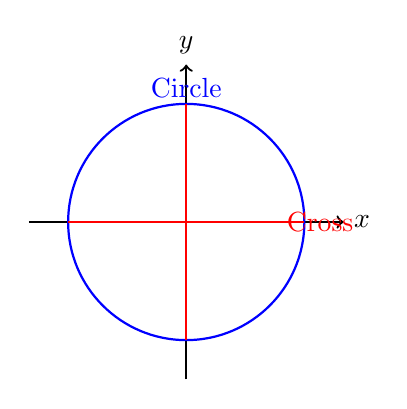
\begin{tikzpicture}
\draw[thick,->] (-2,0) -- (2,0) node[right] {$x$};
\draw[thick,->] (0,-2) -- (0,2) node[above] {$y$};
\draw[thick,blue] (0,0) circle (1.5cm);
\draw[thick,red] (-1.5,0) -- (1.5,0);
\draw[thick,red] (0,-1.5) -- (0,1.5);
\node[blue] at (0,1.7) {Circle};
\node[red] at (1.7,0) {Cross};
\end{tikzpicture}
\caption{A simple TikZ illustration}
\label{fig:tikzsample}
\end{figure}

\lipsum[10-12]

\section{More Tables}
Another table showing multi‑row layout.

\begin{table}[htbp]
\centering
\caption{Multi‑row Table}
\label{tab:multirow}
\begin{tabular}{lll}
\toprule
\textbf{Category} & \textbf{Subcategory} & \textbf{Value} \\
\midrule
A & A1 & 10 \\
  & A2 & 15 \\
B & B1 & 8 \\
  & B2 & 12 \\
  & B3 & 6 \\
C & C1 & 20 \\
\bottomrule
\end{tabular}
\end{table}

\lipsum[13-15]

\section{Additional Lists}
Nested lists example.

\begin{enumerate}
\item Level 1
  \begin{enumerate}
  \item Level 2a
  \item Level 2b
    \begin{itemize}
    \item Level 3 bullet
    \end{itemize}
  \end{enumerate}
\item Another Level 1 item
\end{enumerate}

\lipsum[16-18]

\section{Another Figure}
A second TikZ figure demonstrating a grid.

\begin{figure}[htbp]
\centering
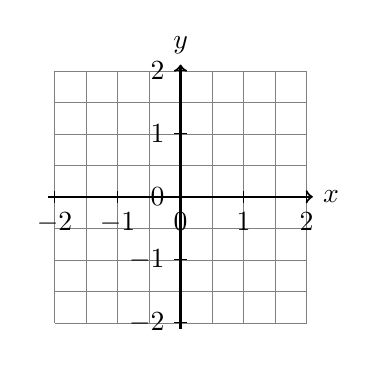
\begin{tikzpicture}[scale=0.8]
\draw[step=0.5cm,gray,very thin] (-2,-2) grid (2,2);
\draw[thick,->] (-2.1,0) -- (2.1,0) node[right] {$x$};
\draw[thick,->] (0,-2.1) -- (0,2.1) node[above] {$y$};
\foreach \x in {-2,-1,...,2}
  \draw (\x,0.1) -- (\x,-0.1) node[below] {$\x$};
\foreach \y in {-2,-1,...,2}
  \draw (0.1,\y) -- (-0.1,\y) node[left] {$\y$};
\end{tikzpicture}
\caption{Coordinate grid}
\label{fig:grid}
\end{figure}

\lipsum[19-21]

\section{Conclusion}
We have shown tables, lists, and figures using TikZ. This document can be extended further as needed.

\end{document}